\renewcommand{\teacherTag}{QUESTION 5 \textbullet\ MANDATORY \textbullet\ 35 MARKS}
\chapter{Signals: Even--Odd Parts, Causality and the Fourier Series}

%------------------------------------------------------------------ 5(a)
\begin{qcard}{Q5(a)}{Sketch and even--odd decomposition}{4 + 8}
Consider the continuous-time signal
\[x(t)=\begin{cases}t+1,&-1\le t\le0,\\[2pt]1-\dfrac t2,&0<t\le2,\\[4pt]0,&\text{otherwise}.\end{cases}\]
(i) Sketch the signal $x(t)$. \ (ii) Decompose $x(t)$ into its even part $x_e(t)$ and odd part $x_o(t)$, analytically or graphically, and sketch $x_e(t)$ and $x_o(t)$.
\end{qcard}
\begin{solution}
\step{(i) The signal.} A triangle: it rises with slope $+1$ from $0$ at $t=-1$ to the peak $1$ at $t=0$, then falls with slope $-\frac12$ to $0$ at $t=2$. (It is continuous: both pieces give $x(0)=1$.)
\begin{center}
\begin{tikzpicture}\begin{axis}[width=8cm,height=4cm,axis lines=middle,xlabel={$t$},ylabel={$x(t)$},xmin=-3,xmax=3.2,ymin=-0.15,ymax=1.3,xtick={-2,-1,0,1,2},ytick={0.5,1},ticklabel style={font=\scriptsize},label style={font=\scriptsize},grid=major,grid style={gray!15}]
\addplot[very thick,navy]coordinates{(-3,0)(-1,0)(0,1)(2,0)(3,0)};
\node[font=\scriptsize,anchor=south east]at(axis cs:-0.5,0.55){slope $1$};\node[font=\scriptsize,anchor=south west]at(axis cs:1,0.55){slope $-\frac12$};
\end{axis}\end{tikzpicture}
\end{center}

\step{(ii) Formulas.} $x_e(t)=\dfrac{x(t)+x(-t)}2$, $\ x_o(t)=\dfrac{x(t)-x(-t)}2$. It is enough to work for $t\ge0$ and then use symmetry ($x_e$ even, $x_o$ odd). For $t\ge0$, $x(-t)$ uses the first piece: $x(-t)=1-t$ for $0\le t\le1$ and $0$ for $t>1$.
\begin{center}\small\renewcommand{\arraystretch}{1.5}\begin{tabular}{@{}c|c|c|c|c@{}}\toprule
interval&$x(t)$&$x(-t)$&$x_e(t)$&$x_o(t)$\\\midrule
$0\le t\le1$&$1-\frac t2$&$1-t$&$1-\frac{3t}{4}$&$\frac t4$\\
$1\le t\le2$&$1-\frac t2$&$0$&$\frac12-\frac t4$&$\frac12-\frac t4$\\
$t\ge2$&$0$&$0$&$0$&$0$\\\bottomrule\end{tabular}\end{center}
For $t<0$: $x_e(t)=x_e(-t)$ and $x_o(t)=-x_o(-t)$. In full:
\[x_e(t)=\begin{cases}1-\frac34\abs t,&\abs t\le1\\[2pt]\frac12-\frac{\abs t}4,&1\le\abs t\le2\\[2pt]0,&\abs t\ge2\end{cases}\qquad
x_o(t)=\begin{cases}\frac t4,&\abs t\le1\\[2pt]\sgn(t)\Big(\frac12-\frac{\abs t}4\Big),&1\le\abs t\le2\\[2pt]0,&\abs t\ge2\end{cases}\]
Key values: $x_e(0)=1$, $x_e(\pm1)=\frac14$, $x_e(\pm2)=0$; $\ x_o(0)=0$, $x_o(\pm1)=\pm\frac14$, $x_o(\pm2)=0$.
\begin{center}
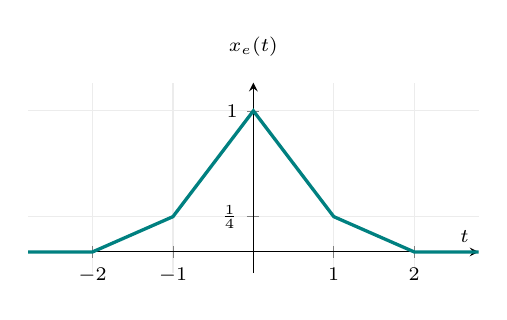
\begin{tikzpicture}\begin{axis}[width=7.3cm,height=4cm,axis lines=middle,xlabel={$t$},title={$x_e(t)$},xmin=-2.8,xmax=2.8,ymin=-0.15,ymax=1.2,xtick={-2,-1,1,2},ytick={0.25,1},yticklabels={$\frac14$,$1$},ticklabel style={font=\scriptsize},label style={font=\scriptsize},title style={font=\scriptsize},grid=major,grid style={gray!15}]
\addplot[very thick,teal]coordinates{(-2.8,0)(-2,0)(-1,0.25)(0,1)(1,0.25)(2,0)(2.8,0)};
\end{axis}\end{tikzpicture}\hspace{2mm}
\begin{tikzpicture}\begin{axis}[width=7.3cm,height=4cm,axis lines=middle,xlabel={$t$},title={$x_o(t)$},xmin=-2.8,xmax=2.8,ymin=-0.4,ymax=0.4,xtick={-2,-1,1,2},ytick={-0.25,0.25},yticklabels={$-\frac14$,$\frac14$},ticklabel style={font=\scriptsize},label style={font=\scriptsize},title style={font=\scriptsize},grid=major,grid style={gray!15}]
\addplot[very thick,coral]coordinates{(-2.8,0)(-2,0)(-1,-0.25)(0,0)(1,0.25)(2,0)(2.8,0)};
\end{axis}\end{tikzpicture}
\end{center}
\step{Check.} $x_e+x_o$ on $0\le t\le1$: $1-\frac{3t}4+\frac t4=1-\frac t2$ \checkmark; on $-1\le t\le0$: $1-\frac34(-t)+\frac t4=1+t$ \checkmark; on $1\le t\le2$: $2(\frac12-\frac t4)=1-\frac t2$ \checkmark; on $-2\le t\le-1$: $(\frac12+\frac t4)-(\frac12+\frac t4)=0$ \checkmark.
\ans{$x_e(t)$: triangle-like even signal with $x_e(0)=1$, $x_e(\pm1)=\frac14$, zero for $\abs t\ge2$; $\ x_o(t)$: odd signal rising linearly to $\frac14$ at $t=1$, back to 0 at $t=2$ (mirrored negative for $t<0$).}
\end{solution}

%------------------------------------------------------------------ 5(b)
\begin{qcard}{Q5(b)}{Minimum shift for causality}{6}
Let $x(t)=e^{-3t}u(t+3)$ and $y(t)=x(t-a)$. Identify the minimum value of $a$ for which $y(t)$ is a causal signal.
\end{qcard}
\begin{solution}
\step{Step 1 --- Support of $x$.} $u(t+3)=1$ for $t\ge-3$, so $x(t)\ne0$ for $t\ge-3$: $x$ starts at $t=-3$ (with value $e^{9}$) and is \emph{not} causal.

\step{Step 2 --- Support of $y$.} $y(t)=x(t-a)=e^{-3(t-a)}u(t-a+3)$ is non-zero for $t-a+3\ge0$, i.e.\ $t\ge a-3$.

\step{Step 3 --- Causal condition.} A causal signal is zero for $t<0$, so we need $a-3\ge0$:
\[a\ge3\quad\Longrightarrow\quad a_{\min}=3,\qquad y(t)=e^{-3(t-3)}u(t)=e^{9}e^{-3t}u(t).\]
\begin{center}
\begin{tikzpicture}\begin{axis}[width=7.6cm,height=3.8cm,axis lines=middle,xlabel={$t$},xmin=-4.2,xmax=2.5,ymin=0,ymax=1.25,xtick={-3,0,1,2},ytick=\empty,ticklabel style={font=\scriptsize},label style={font=\scriptsize},legend style={font=\scriptsize,draw=none,at={(0.98,0.98)},anchor=north east}]
\addplot[very thick,slate,dashed,domain=-3:2,samples=80]{exp(-3*(x+3))};\addlegendentry{$x(t)$ (starts at $-3$)}
\addplot[very thick,navy,domain=0:2,samples=80]{exp(-3*x)};\addlegendentry{$y(t)=x(t-3)$}
\addplot[thick,slate,dashed]coordinates{(-3,0)(-3,1)};\addplot[thick,navy]coordinates{(0,0)(0,1)};
\end{axis}\end{tikzpicture}
\end{center}
{\small(Heights normalised: both curves start at $e^{9}$; the shift moves the starting edge from $t=-3$ to $t=0$.)}
\ans{$a_{\min}=3$ (a delay of 3 moves the starting point $t=-3$ to $t=0$).}
\end{solution}

%------------------------------------------------------------------ 5(c)
\begin{qcard}{Q5(c)}{Can a causal impulse response be periodic?}{5}
Consider an LTI system with impulse response $h(t)$. If the system is causal, can $h(t)$ be periodic? Explain your answer.
\end{qcard}
\begin{solution}
Causal means $h(t)=0$ for all $t<0$. Suppose $h$ is also periodic with some period $T>0$: $h(t)=h(t-nT)$ for every integer $n$.

Take any time $t$. Choose $n$ so large that $t-nT<0$. Then
\[h(t)=h(t-nT)=0\quad(\text{causality}).\]
Since $t$ was arbitrary, $h(t)=0$ for all $t$. So the only causal periodic impulse response is the trivial one, $h\equiv0$ (a system that outputs nothing).

Intuition: periodicity forces the ``past'' $t<0$ to repeat the ``future'' $t>0$, while causality forces the past to be zero; both can hold only if everything is zero. (Also, a non-zero periodic $h$ is never absolutely integrable, so it could not be stable either.)
\ans{No. A causal and periodic $h(t)$ must be identically zero: for any $t$, $h(t)=h(t-nT)$ with $t-nT<0$, which is 0 by causality.}
\end{solution}

%------------------------------------------------------------------ 5(d)
\begin{qcard}{Q5(d)}{Complex exponential Fourier series}{12}
Consider the continuous-time periodic signal
\[x(t)=4+\sin\!\Big(\omega_0t-\frac\pi4\Big)+2\cos(3\omega_0t).\]
Express $x(t)$ in complex exponential Fourier series form, and relate each non-zero coefficient to the corresponding frequency component of $x(t)$.
\end{qcard}
\begin{solution}
\step{Step 1 --- Use Euler's formulas} $\sin\theta=\dfrac{e^{j\theta}-e^{-j\theta}}{2j}$ and $\cos\theta=\dfrac{e^{j\theta}+e^{-j\theta}}{2}$. No integration is needed.
\[\sin\!\Big(\omega_0t-\frac\pi4\Big)=\frac{e^{-j\pi/4}}{2j}e^{j\omega_0t}-\frac{e^{j\pi/4}}{2j}e^{-j\omega_0t},\qquad 2\cos3\omega_0t=e^{j3\omega_0t}+e^{-j3\omega_0t}.\]
\step{Step 2 --- Simplify the coefficients.} With $\frac1j=e^{-j\pi/2}$:
\[a_1=\frac{e^{-j\pi/4}}{2j}=\frac12e^{-j3\pi/4}=-\frac{\sqrt2}{4}(1+j),\qquad a_{-1}=-\frac{e^{j\pi/4}}{2j}=\frac12e^{j3\pi/4}=-\frac{\sqrt2}{4}(1-j)=a_1^* .\]
\step{Step 3 --- The series.}
\[\boxed{x(t)=4+\tfrac12e^{-j3\pi/4}e^{j\omega_0t}+\tfrac12e^{j3\pi/4}e^{-j\omega_0t}+e^{j3\omega_0t}+e^{-j3\omega_0t}}\]
\begin{center}\small\renewcommand{\arraystretch}{1.35}\begin{tabular}{@{}c|c|c|c|l@{}}\toprule
$k$&$a_k$&$\abs{a_k}$&$\angle a_k$&frequency component\\\midrule
$0$&$4$&$4$&$0$&d.c.\ (average) value $4$\\
$\pm1$&$\frac12e^{\mp j3\pi/4}$&$\frac12$&$\mp135^\circ$&fundamental $\omega_0$: $2\abs{a_1}\cos(\omega_0t+\angle a_1)=\cos(\omega_0t-\tfrac{3\pi}4)=\sin(\omega_0t-\tfrac\pi4)$\\
$\pm3$&$1$&$1$&$0$&third harmonic $3\omega_0$: $2\abs{a_3}\cos3\omega_0t=2\cos3\omega_0t$\\
others&$0$&$0$&--&absent (no 2nd, 4th, \dots\ harmonic)\\\bottomrule\end{tabular}\end{center}
\step{Step 4 --- How the coefficients relate to the components.} Each real sinusoid $A\cos(k\omega_0t+\theta)$ splits into a conjugate pair $a_{\pm k}=\frac A2e^{\pm j\theta}$: the \emph{magnitude} $\abs{a_k}$ is half the amplitude, the \emph{angle} is the phase, and $a_{-k}=a_k^*$ because $x$ is real. The constant term is $a_0$.
\begin{center}
\begin{tikzpicture}\begin{axis}[width=7.2cm,height=4cm,axis lines=middle,xlabel={$k$},title={$\abs{a_k}$},xtick={-3,-2,-1,0,1,2,3},ymin=0,ymax=4.6,xmin=-3.8,xmax=3.8,ticklabel style={font=\scriptsize},label style={font=\scriptsize},title style={font=\scriptsize}]
\addplot+[ycomb,navy,thick,mark=*,mark size=1.6pt]coordinates{(-3,1)(-1,0.5)(0,4)(1,0.5)(3,1)};
\end{axis}\end{tikzpicture}\hspace{2mm}
\begin{tikzpicture}\begin{axis}[width=7.2cm,height=4cm,axis lines=middle,xlabel={$k$},title={$\angle a_k$ (degrees)},xtick={-3,-1,1,3},ytick={-135,135},ymin=-170,ymax=170,xmin=-3.8,xmax=3.8,ticklabel style={font=\scriptsize},label style={font=\scriptsize},title style={font=\scriptsize}]
\addplot+[ycomb,crimson,thick,mark=*,mark size=1.6pt]coordinates{(-1,135)(1,-135)};
\addplot+[only marks,crimson,mark=*,mark size=1.6pt]coordinates{(-3,0)(0,0)(3,0)};
\end{axis}\end{tikzpicture}
\end{center}
\step{Check (Parseval).} $\sum\abs{a_k}^2=16+2(\tfrac14)+2(1)=18.5$, and the average power directly: $4^2+\frac{1^2}2+\frac{2^2}2=18.5$ \checkmark.
\ans{$a_0=4$, $a_{\pm1}=\frac12e^{\mp j3\pi/4}$, $a_{\pm3}=1$, all others $0$: $a_0$ is the d.c.\ level, $a_{\pm1}$ the fundamental $\sin(\omega_0t-\pi/4)$ (amplitude $2\abs{a_1}=1$, phase $-135^\circ$ as a cosine) and $a_{\pm3}$ the third harmonic $2\cos3\omega_0t$.}
\end{solution}
